\chapter{Semiconductor model}

In this chapter we shall present the basic physics properties of semiconductor material accordingly with the quantum mechanics theory \citep{ModernVLSIdevices}. The Drift-Diffusion model is then presented.

\section{Basic Device Physics}

This section covers the basic concepts of semiconductor device physics. As the most used material in the fabrication of VLSI devices is silicon, in the follow we will focus on it.

\subsection{Intrinsic semiconductor}
In a silicon crystal each atom has four valence electrons to share with its four nearest neighboring atoms. The valence electrons are shared in a paired configuration called a covalent bond. The most important result of the application of quantum mechanics to the description of electrons in a solid is that the allowed energy levels of electrons are grouped into bands. The bands are separated by regions of energy that the electrons in the solid cannot possess: forbidden gaps. The highest energy band that is completely filled by electron at 0[K] is called the \textit{valence band} ($E_V$). The next higher energy band, separated by a frobidden gap from the valence band, is called the \textit{conduction band} ($E_C$).

\begin{figure}[!h]
\centering
\subfloat[][Metal]
{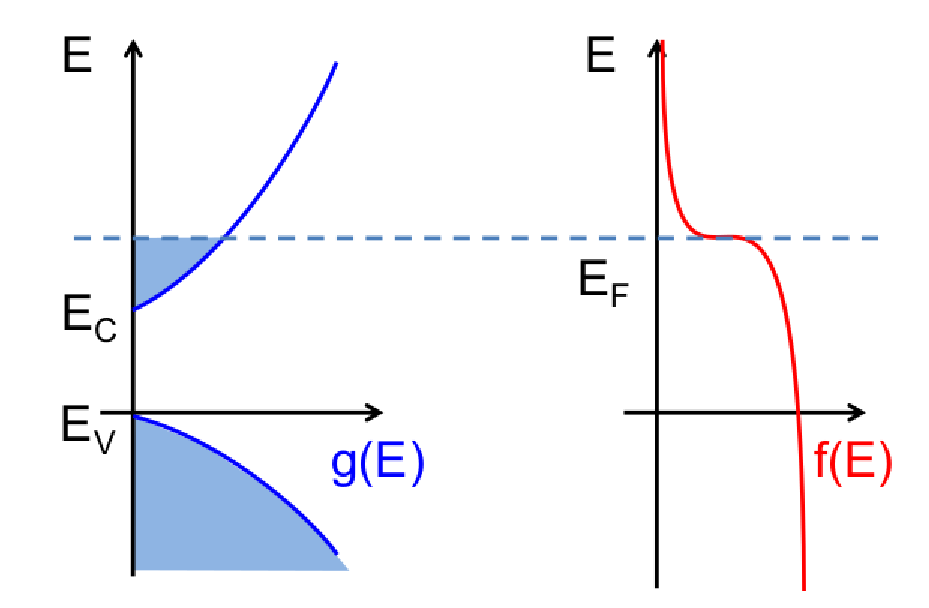
\includegraphics[width=.45\textwidth]{SemiconductorModel/BandeMetalli.eps}}
\psp{5}
\subfloat[][Insulator]
{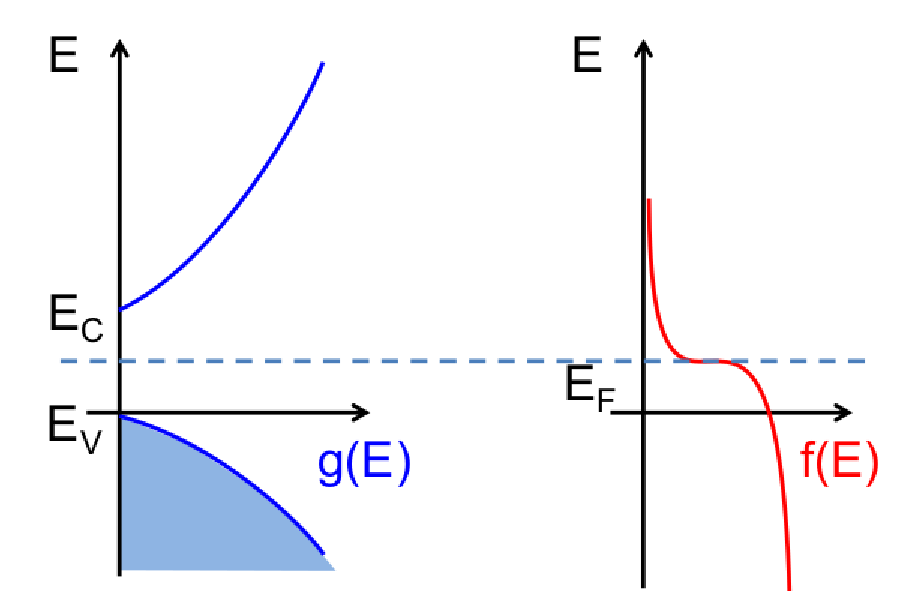
\includegraphics[width=.45\textwidth]{SemiconductorModel/BandeSemiconduttori.eps}}
\caption{Two typical examples of state density occupation (g(E)) and probability distribution (f(E)).  }
\end{figure}

Because in silicon the band gap is on the order of 1 [eV], at room temperature a small fraction of the electrons are excited into the conduction band, leaving behind vacancies (called \textit{holes}) in the valence band.
In contrast, an insulator has a much larger forbidden gap making room-temperature conduction virtually impossible, while metals have partially filled conduction bands even at absolute zero temperature, this make them good conductors at any temperature. 

A suitable formulation of che carrier concentration which is given, for electrons, by the follow integral:
\begin{equation}
\label{eq: carrier densiy integral}
n = \int_{E_c}^\infty g(E)f(E) \, dE
\end{equation}
With $g(E)dE$ we indicate the number of electronic states per unit volume with an energy between $E$ and $E+dE$ in the conduction band and $f(E)$ is a suitable probability ditribution.

The energy distribution of electrons in a solid is governed by the laws of Fermi-Dirac statistics. For a system in thermal equilibrium, the principal result of these statistics is the \textit{Fermi-Dirac distribution function}, which gives the probability that an electronic state at energy E is occupied by an electron,
\begin{equation}
\label{eq: fermi dirac distribution}
f_D(E) = \dfrac{1}{1+exp\left(\dfrac{E-E_f}{k_BT}\right)} 
\end{equation}
here $k_B=1.38\times10^{-23}[J/K]$ is Boltzmann's constant, $T$ is the absolute temperature and $E_f$ is the \textit{Fermi level}.

\begin{Definizione}
The Fermi level ($E_f$) is the energy at which the probability of occupation of an energy state by an electron is exactly one-half.
\end{Definizione}

In most cases when the energy is at least several $k_BT$ above or below the Fermi level \referenzaeq{eq: fermi dirac distribution} can be approximated with the Maxwell-Boltzmann statistics for classical particles, which read as follows:

\begin{equation}
\label{eq: maxwell distribution}
f_D(E)\simeq f_{MB}(E) = 
\begin{cases}
exp\left(-\dfrac{E-E_f}{KT}\right) & E\gg E_f \\
1-exp\left(-\dfrac{E_f-E}{KT}\right) & E \ll E_f
\end{cases}
\end{equation}

Fermi level plays an essential role in characterizing the equilibrium state of a stystem, it is important to keep in mind the sequent observation.

\begin{Osservazione}
When two systems are in thermal equilibrium with no current flow between them, their Fermi levels must be equal, in other words for a continuous region of metals and/or semiconductors in contact, the Fermi level at thermal equilibrium is flat (spatially constant throughout the region).
\end{Osservazione}

 In general \referenzaeq{eq: carrier densiy integral} is a Fermi integral of the order $1/2$ and must be evaluated numerically. In the case of non-degenerate semiconductor, Fermi levels stay at least $3KT/q$ below the edge of the conduction band (for holes we consider the same approximation above the valence band).  The Fermi-Dirac distribution can be approximated by the Maxwell-Boltzmann distribution and \referenzaeq{eq: carrier densiy integral} can be solved in the analytically way, obtaining,

\begin{align}
n & = N_c exp\left(-\dfrac{E_c-E_f}{KT}\right) \label{eq: n density fd}\\
p & = N_v exp\left(-\dfrac{E_f-E_v}{KT}\right)  \label{eq: p density fd}
\end{align}

where $N_c$ and $N_v$ are the \textit{effective density of states}.
In intrisic semiconductor $n=p$ and the \textit{intrinsic Fermi level} $E_i$ can be calculated using equations \referenzaeq{eq: n density fd} and \referenzaeq{eq: p density fd} as:

\begin{equation}
\label{eq: midgap equilibrium}
E_i=E_f=\dfrac{E_c+E_v}{2} - \dfrac{KT}{2}ln\left(\dfrac{N_c}{N_v}\right)
\end{equation}

By replacing \referenzaeq{eq: midgap equilibrium} in \referenzaeq{eq: n density fd} we have the expression of the intrinsic carrier concentration $n_i=n=p$:


\begin{equation}
\label{eq: ni equilibrium NcNv}
n_i = \sqrt{N_cN_v}exp\left(-\dfrac{E_g}{2KT}\right)
\end{equation}

\begin{Osservazione}
Since the thermal energy, $k_BT$ is muc smaller than the usual semiconductor bandgap $E_g$, the intrinsic Fermi level is very close to the midpoint between the conduction band and the valence band.
\end{Osservazione}

Equations \referenzaeq{eq: n density fd} and \referenzaeq{eq: p density fd} can be rewritten in terms of the intrinsic carrier density ($n_i$) and energy ($E_i$) :

\begin{align}
n & = n_i exp\left(\dfrac{E_f-E_i}{KT}\right) \label{eq: n density mb}\\
p & = n_i exp\left(\dfrac{E_i-E_f}{KT}\right)  \label{eq: p density mb}
\end{align}

Finally we remark a fundamental and useful relation holds at the thermical equilibrium

\begin{equation}
\label{eq: legge di azione di massa}
np=n_i^2
\end{equation}

this relation is usually note as \textit{mass action law}.

One of the most used graphical tool for the anlysis of the functionality of devices is the band diagram \figref{fig: band diagram}, which summarizes the informations presented above.
\begin{figure}[!h]
\centering
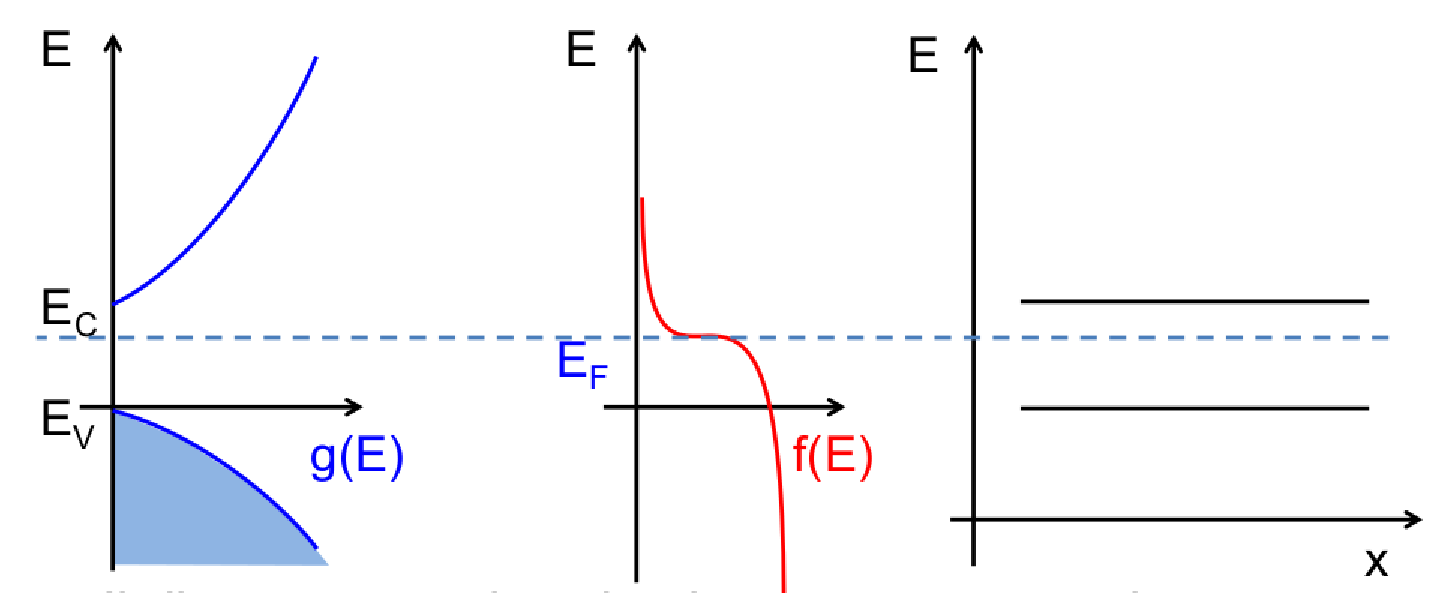
\includegraphics[width=.8\textwidth]{SemiconductorModel/DiagrammaBande.eps}
\caption{Construction of tha band diagram.}
\label{fig: band diagram}
\end{figure}

\subsection{Extrinsic semiconductor}
At room temperature intrinsic semiconductor has an extremely low free-carrier concentration, therefore, its resistivity is very high. In order to make semiconductor a better conductor it's usual add impurities atoms which introduce additional energy levels in the forbidden gap: these impurities are easily ionized adding either electrons to the conduction band or holes to the valence band. Here the electrical conductivity is dominated by the type and concentration of the impurity atoms.

In the case of silicon two are the types of impurities which are electrically active: those from column V such as arsenic or phosphorus, and those from column III such as boron or indium.

A column-V atom in a silicon lattice tends to have one extra electron loosely bonded after forming covalent bonds with other silicon atoms. In most cases, the thermal energy at room temperature is sufficient to ionize the impurity atom and free the extra electron to the conduction band. Such type of impurities are called \textit{donors}; they become positively charged when ionized. Silicon material doped with column-V impurities or donors is called \textit{n-type} silicon.

A column-III impurity atom in a silicon lattice tends to be deficient by one electron when forming covalent bonds with other silicon atoms. Such an impurity atom can also be ionized by accepting an electron from the valence band, which leaves a free-moving hole that contributes to electrical conduction. These impurities are called \textit{acceptors}: they become negatively charged when ionized. Silicon material doped with column-III impurities or acceptors is called \textit{p-type} silicon.

A p-type or an n-type is named as \textit{extrinsic} silicon.
In terms of the energy-band diagrams, donors add allowed electron states in the bandgap close to the conduction-band edge, while acceptors add allowed states just above the valence-band edge.

In contrast to intrinsic silicon, the Fermi level in an extrinsic silicon is not located at the midgap. The Fermi level in n-type silicon moves up towards the conduction band while in p-type silicon moves down towards the valence band.
The exact position of the Fermi level depends on both the ionization energy and the concentration of dopants. For example, for an n-type material with a donor impurity concentration, $N_d$, the charge neutrality condition requires that
\begin{equation}
\label{eq: equilibrium charge in n-type}
n = N_d^+ + p
\end{equation}
 where $N_d^+$ is the density of ionized donors.  Similarly for a p-type material with acceptor impurity concentration $N_a$ we have
\begin{equation}
\label{eq: equilibrium charge in p-type}
p = N_a^- + n
\end{equation}
 
 For the sake of simplicity we consider in this work that at room temperature all impurties are ionized ($N_d = N_d^+$ and $N_a = N_a^-$). Typcally the magnitude of impurities is between $10^{16}\ast 10^{20} [cm^{-3}]$, while the usual intrinsic carrier concentration is almost $10^{10}[cm_3]$, for this reason we can approximate the equilibrium densities concentration:
  
\begin{equation}
\begin{array}{ll}
n \simeq N_d & p \simeq \dfrac{n_i^2}{N_d} \\ \\
p \simeq N_a & n \simeq \dfrac{n_i^2}{N_a}
\end{array}
\end{equation}

 Take into account this approximation and substituting \referenzaeq{eq: n density fd} and \referenzaeq{eq: p density fd} in \referenzaeq{eq: equilibrium charge in n-type} and \referenzaeq{eq: equilibrium charge in p-type}, solving the algebraic equationwe have
 
 \begin{align}
 E_c-E_f = KTln\left(\dfrac{N_c}{N_d}\right)  \label{eq: Ef in n-type}\\
 E_f-E_v= KTln\left(\dfrac{N_v}{N_a}\right) \label{eq: Ef in p-type}
 \end{align}

Equation \referenzaeq{eq: legge di azione di massa} is indipendent of the dopant type and Fermi level position.
Instead of using $N_c$, $N_v$ and referring to $E_c$ and $E_v$ equation \referenzaeq{eq: Ef in n-type} and \referenzaeq{eq: Ef in p-type} can be written in a more useful form in terms of $n_i$ and $E_i$ defined by equations \referenzaeq{eq: ni equilibrium NcNv} and \referenzaeq{eq: midgap equilibrium}:

 \begin{align}
 E_f-E_i = KTln\left(\dfrac{N_d}{n_i}\right)  \label{eq: Ef in n-type Ei} \\
 E_i-E_f = KTln\left(\dfrac{N_a}{n_i}\right)  \label{eq: Ef in p-type Ei} 
 \end{align}

\begin{Osservazione}
The distance between the Fermi level and the intrinsic Fermi level near the midgap is a logarithmic function of doping concentration.
\end{Osservazione}

As a consequences:
\begin{itemize}
\item non linearity relations between potential and desities,
\item exponential dependence of densities from potential.
\end{itemize}

\begin{figure}[!h]
\centering
\subfloat[][n-type]
{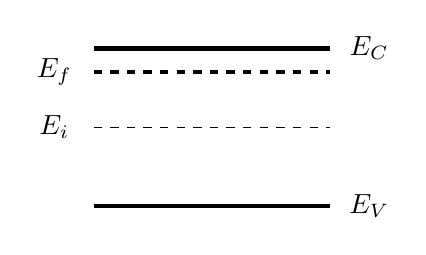
\begin{tikzpicture}
[scale=1.0]
\def\Ecxa{0.0}
\def\Ecya{2}
\def\Ecxb{3}
\def\Ecyb{2}

\def\Evxa{\Ecxa}
\def\Evya{0}
\def\Evxb{\Ecxb}
\def\Evyb{0}

\def\Efxa{\Ecxa}
\def\Efya{1.7}
\def\Efxb{\Ecxb}
\def\Efyb{1.7}

\def\Eixa{\Ecxa}
\def\Eiya{1}
\def\Eixb{\Ecxb}
\def\Eiyb{1}

\node at (\Ecxb+0.5,\Ecyb){$E_C$};
\node at (\Evxb+0.5,\Evyb){$E_V$};
\node at (\Efxa-0.5,\Efya){$E_f$};
\node at (\Eixa-0.5,\Eiya){$E_i$};

\draw[ultra thick](\Ecxa,\Ecya)--(\Ecxb,\Ecyb);
\draw[ultra thick](\Evxa,\Evya)--(\Evxb,\Evyb);
\draw[ultra thick,dashed](\Efxa,\Efya)--(\Efxb,\Efyb);
\draw[dashed](\Eixa,\Eiya)--(\Eixb,\Eiyb);
\end{tikzpicture}}
\psp{20}
\subfloat[][p-type]
{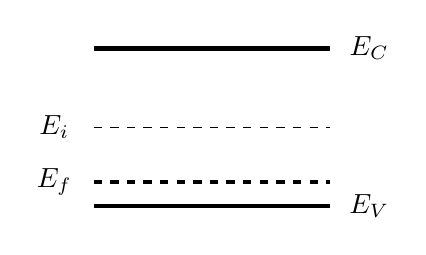
\begin{tikzpicture}
[scale=1.0]
\def\Ecxa{0.0}
\def\Ecya{2}
\def\Ecxb{3}
\def\Ecyb{2}

\def\Evxa{\Ecxa}
\def\Evya{0}
\def\Evxb{\Ecxb}
\def\Evyb{0}

\def\Efxa{\Ecxa}
\def\Efya{0.3}
\def\Efxb{\Ecxb}
\def\Efyb{0.3}

\def\Eixa{\Ecxa}
\def\Eiya{1}
\def\Eixb{\Ecxb}
\def\Eiyb{1}

\node at (\Ecxb+0.5,\Ecyb){$E_C$};
\node at (\Evxb+0.5,\Evyb){$E_V$};
\node at (\Efxa-0.5,\Efya){$E_f$};
\node at (\Eixa-0.5,\Eiya){$E_i$};

\draw[ultra thick](\Ecxa,\Ecya)--(\Ecxb,\Ecyb);
\draw[ultra thick](\Evxa,\Evya)--(\Evxb,\Evyb);
\draw[ultra thick,dashed](\Efxa,\Efya)--(\Efxb,\Efyb);
\draw[dashed](\Eixa,\Eiya)--(\Eixb,\Eiyb);
\end{tikzpicture}}
\caption{Band diagrams of estrinsic silicon.}
\label{fig: Band diagrams of estrinsic silicon}
\end{figure}

\subsection{Densities at nonequilibrium condition}

In VLSI device operation a nonequilibrium sistuations is often possible: the densities of one or both types of carriers depart from their equilibrium values given by \referenzaeq{eq: n density mb} and \referenzaeq{eq: p density mb}.
In particular, the minority carrier concentration can be easily overwhelmed by injection from neighboring regions. Under these circumstances, while the electrons and holes are in local equilibrium with themselves, they are not in equilibrium with each other. In order to extend the relationship between Fermi level and densities discussed above, we can introduce separate Fermi levels for electrons and holes. They are called \textit{quasi Fermi levels} defined as $E_{fn}$ and $E_{fp}$ replacing equation \referenzaeq{eq: n density mb} and \referenzaeq{eq: p density mb}:

\begin{align}
n & = n_i exp\left(\dfrac{E_{fn}-E_i}{k_BT}\right) \label{eq: non eq n density mb}\\
p & = n_i exp\left(\dfrac{E_i-E_{fp}}{k_BT}\right)  \label{eq: non eq p density mb}
\end{align}

In non equilibrium condition quasi Fermi levels have a similar physical interpretation in terms of the state occupancy as the Fermi level.
\begin{Osservazione}
The electron density in the conduction band can be calculated using $E_{fn}$, and the hole density in the valence band using $E_{fp}$.
\end{Osservazione}

\subsection{Carrier transport in semiconductor}
\label{sec: carrier transport}

Carrier transport or current flow in silicon is driven by two different mechanisms:
\begin{itemize}
\item the \textbf{drift} of carriers, which is caused by the presence of an electric field;
\item the \textbf{diffusion} of carriers, which is caused by and electron or hole concentration gradient.
\end{itemize}

\subsubsection{Drif current - Ohm's law}

When an electric field is applied to a media, the free carriers are accelerated and acquire a drift velocity superimposed upon their random thermal motion.

\begin{Osservazione}
The drift velocity of holes ($h$) is in the direction of the applied field, and the drift velocity of electrons ($e$) is opposite to the field.
\end{Osservazione}

The velocity of the carriers does not increase indefinitely under field acceleration, since they are scattered frequently and lose their acquired momentum after each collision.
During their motion throughout the lattice structure, carriers travel at an average speed definded as
\begin{equation}
\label{eq: velocities}
\vect{v}_d^e = - \dfrac{q\vect{E}\tau_e}{m_e}  \psp{20} 
\vect{v}_d^h = + \dfrac{q\vect{E}\tau_h}{m_h}
\end{equation}

where $q=1.602e^{-19}[C]$ is the elementary charge, $\vect{E}$ the electric field, $\tau_\eta$ the average time of flight of the carrier between two consecutive interactions with the atoms of the lattice and $m_\eta$ is the effective mass.
The coefficient $q\tau_\eta / m_\eta$ characterizes how quickly a carrier can move through the lattice and it's well known as carrier mobility $[m^2V^{-1}s^{-1}]$.
In general, to include different contributions to the mobility \textit{Matthiessen's rule} is used:
\begin{equation}
\dfrac{1}{\mu} = \dfrac{1}{\mu_L} + \dfrac{1}{\mu_I} + \cdots
\end{equation}
where $\mu_L$ and $\mu_I$ correspond to the lattice and impurity scattering limited components of mobility (for a more detailed description of mobility models see \cite{ModernVLSIdevices}). 

Therefore the drift electron, hole, current density, reads as follows:

\begin{align}
\vect{J}_n =& -qn\vect{v}_d^n = qn\mu_n\vect{E}   = \sigma_n\vect{E} \label{eq: drift electron} \\ 
\vect{J}_p =& +qp\vect{v}_d^p = qp\mu_p\vect{E} = \sigma_p\vect{E} \label{eq: drift hole}
\end{align}

The scalar coefficient $qn\mu_n(qp\mu_p)$ is often summerized by the electron (hole) conductivity $\sigma_n(\sigma_p)$. 

Relations \referenzaeq{eq: drift electron} and \referenzaeq{eq: drift hole} expresses the well known \textit{Ohm' law} stating that the current density is directly proportional to the applied electric field.


\subsubsection{Diffusion current - Fick's law}

In semiconductor devices it's usual have different profiles of dopant in order to allow particular behaviors, this implies a not uniform concentration of carriers which they also diffuse as a result of the concentration gradient. This leads to an additional current contribution accordingly to the \textit{Fick's law}:
\begin{align}
\vect{J}_n = -D_n(-q\nabla n) \label{eq: diff electron}\\
\vect{J}_p = -D_p(+q\nabla p) \label{eq: diff hole}
\end{align}

The proportionally constants $D_n$ and $D_p$ are called the electron and hole diffusion coefficients and have units of $[cm^2s^{-1}]$. Physically, both drift and diffusion are closely associated with the random thermal motion of carriers and their collisions with the silicon lattice in thermal equilibrium. A simple relationship between the diffusion coefficient and the mobility is the well known \textit{Einstein relation}:
\begin{equation}
D_\eta = \dfrac{k_BT}{q}\mu_\eta
\end{equation}

\subsubsection{Drift-Diffusion transport equations}
\label{subsub:driftdiffusion transport}

By considering \referenzaeq{eq: drift electron}, \referenzaeq{eq: drift hole}, \referenzaeq{eq: diff electron} and \referenzaeq{eq: diff hole}, the total electron and hole current densities are:

\begin{align}
\vect{J}_n &= qn\mu_n\vect{E} + qD_n\nabla n  \label{eq: drift diff electron}\\ 
\vect{J}_p &= qp\mu_p\vect{E} - qD_p \nabla p \label{eq: drift diff hole}
\end{align}
The total conduction current density is $\vect{J}=\vect{J}_n+\vect{J}_p$.

We remark that these constitutive laws can be rewritten in two other ways highlighting different physical explanations of the same phenomenon. Moreover these reinterpreations  give different start points for the discrete solver algorithm.

Considering that electric field is related to the scalar potential as:
\begin{equation}
\label{eq: relazione pot electric}
\vect{E}  = -\nabla \varphi
\end{equation}

the current densities can be :

\begin{align}
\vect{J}_n &= -qn\mu_n\left(\nabla \varphi - \dfrac{k_BT}{qn}\nabla n \right) \label{eq: Jn DD} \\ 
\vect{J}_p &= -qp\mu_p\left(\nabla \varphi+ \dfrac{k_BT}{qp} \nabla p \right) \label{eq: Jp DD}
\end{align}

Considering equations \referenzaeq{eq: non eq n density mb} and \referenzaeq{eq: non eq p density mb} the above can be written as:

\begin{align}
\vect{J}_n = -qn\mu_n\nabla \varphi_n \label{eq: Jn qf}\\
\vect{J}_p = -qp\mu_p\nabla \varphi_p \label{eq: Jp qf}
\end{align}

With these equations we underlying an important aspect which occur in semiconductor material:
\begin{Osservazione}
The current density is proportional to the gradient of the quasi Fermi potential.
\end{Osservazione}

The third way to represent the current density is based on \textit{Slotboom variables}. In 1973 Jan Slotboom proposed this change in variables for the two-dimensional numercal simulation of a bipolar transistor:

\begin{align}
u_n &= n_iexp\left(-\dfrac{\varphi_n}{V_{th}} \right) \label{eq: un slotboom} \\
u_p &= n_iexp\left(\dfrac{\varphi_p}{V_{th}} \right) \label{eq: up slotboom} 
\end{align}

where $V_{th}=k_BT/q$. Using the above equations into \referenzaeq{eq: drift diff electron} and \referenzaeq{eq: drift diff hole} we obtain:

\begin{align}
\vect{J}_n &= qD_n exp\left(\dfrac{\varphi}{V_{th}}\right) \nabla u_n \label{eq: Jn slotboom} \\
\vect{J}_p &= -qD_p exp\left(-\dfrac{\varphi}{V_{th}}\right)  \nabla u_p \label{eq: Jp slotboom}
\end{align}

This interpretation results is:
\begin{Osservazione}
The drift-diffusion current density in a semiconductor, is a totally diffusive flux of a new kind of carrier and diffusivity coefficient. 
\end{Osservazione}


\section{Drift Diffusion Model for semiconductor}
\label{section: dd model for semi}

Simulations on integrated devices works on several different scale, the \textit{Drift Diffusion model} (DD) is the most widely used mathematical tool for industrial simulaiton of semiconductor devices. In this section we'll show how is possible to deduce the DD model.

\subsection{Drift Diffusion formulation}
 The system of Maxwell equations describes the propagation of electromagnetic signal in a medium:

\begin{align}
\nabla \times \vect{H} & =  \vect{J} + \dfrac{\partial \vect{D}}{\partial t} \label{eq: magnetic equation} \\ 
\nabla \times \vect{E} & =  - \dfrac{\partial \vect{B}}{\partial t} \label{eq: ampere law}\\ 
\nabla \cdot \vect{D} & =  \rho \label{eq: gauss law}\\ 
\nabla \cdot \vect{B} &  =  0 \label{eq: no magetic charge law}
\end{align}

we complete the system with the following set of constitutive laws that characterize the electromagnetic properties of the medium:

\begin{equation}
\begin{array}{rcl}
\vect{D} & = & \epsilon \vect{E} \\
\vect{B} & = & \mu_m \vect{H} \label{eq: magnetic costitutive}
\end{array}
\end{equation}

where $\epsilon$ is the material dielectric permettivity $[F cm^{-1}]$ and $\mu_m$ is the magnetic permeability $[H cm^{-1}]$. Since $\nabla \cdot (\nabla \times \vect{A})=0$ for any vector $\vect{A}$, \referenzaeq{eq: no magetic charge law} is satisfied by introducing a vector potential $\vect{A}$ such that $\vect{B}= \nabla \cdot \vect{A}$. We replace it in \referenzaeq{eq: ampere law} and we obtain

\begin{equation}
\nabla \times \left( \vect{E} + \dfrac{\partial \vect{A}}{\partial t} \right) = 0.
\end{equation}

From this we can state that exist a scalar potential $\varphi$ such that

\begin{equation}
\label{eq: potenziale scalare}
\vect{E} + \dfrac{\partial \vect{A}}{\partial t} = -\nabla \varphi
\end{equation}


We multiply \referenzaeq{eq: potenziale scalare} by $\epsilon$, we apply the divergence operator and we obtain using \referenzaeq{eq: relazione pot electric}, \referenzaeq{eq: magnetic costitutive} and \referenzaeq{eq: gauss law}

\begin{equation}
\rho + \dfrac{\partial \vect{A}}{\partial t}  = -\nabla \cdot (\epsilon \nabla \varphi)
\end{equation}

We now assume that $\dfrac{\partial \vect{A}}{\partial t} = 0$ (quasi static approximation) and we obtain the \textit{Poisson Equation}

\begin{equation}
\label{eq: Poisson equation}
\nabla \cdot (\epsilon \nabla \varphi) = \rho.
\end{equation} 
	
	We apply the divergence operator on the equation \referenza{eq: magnetic equation}  and we get the \textit{Continuity Equation}

\begin{equation}
\dfrac{\partial \rho}{\partial t} + \nabla \cdot \vect{J}  =  0 \end{equation} 




To close the above system we need to specify the mathematical form of the electric charge density ($\rho$) and the electric conduction current density ($\vect{J}$).
As we introduced in the preview section, devices are usually formed by extrinsic semiconductor and this causes the presence in the lattice of two kind of charge:

\begin{itemize}
\item free charge ($\rho_{free}$) (free electron and holes carriers),
\item fixed charge ($\rho_{fixed}$) (ionoized dopant impurities).
\end{itemize} 

\begin{equation}
\label{eq: charge balance}
\rho = \underbrace{q(p-n)}_{\rho_{free}} +\underbrace{q(N_D^+-N_A^-)}_{\rho_{fixed}}
\end{equation}

 Notice that we assume $N_D^+$ and $N_A^-$ time invariant ($\partial N_D^+ / \partial t=\partial N_A^- / \partial t = 0$).

 Accordingly with the preview hypotesis and replacing \referenzaeq{eq: charge balance}, \referenzaeq{eq: drift diff electron} and \referenzaeq{eq: drift diff hole}, we can split the continuity equation into the contribute of electrons and holes, the DD model formulation looks as follows:
 
\begin{equation}
\label{eq: full problem}
\left\{
\begin{array}{rcl}
\nabla \cdot (-\epsilon \nabla \varphi) & = & q(p-n+N_D^+-N_A^-)\\ \\
-q\dfrac{\partial n}{\partial t} + \nabla \cdot ( - q\mu_n n \nabla \varphi + qD_n \nabla n )& = & qR\\ \\
q\dfrac{\partial p}{\partial t} + \nabla \cdot (- q\mu_p p \nabla \varphi - qD_p \nabla p )& = & -qR 
\end{array}
\right.
\end{equation}

The system is an incompletely parbolic initial value/boundary problem in three scalar unkown dependent variables $\varphi(\vect{x},t)$, $n(\vect{x},t)$ and $p(\vect{x},t)$. Notice that the problem is a nonlinearly coupled system of PDE's, because of the presence of the drift terms ($n\nabla \varphi$ and $p \nabla 	\varphi$). 

From Maxwell equations we are able to guarantee only that $\vect{J}$ is a solenoidal field, we can't say nothing about the properties of $\vect{J_n}$ and $\vect{J_p}$. We can interpret $R(\vect{x},t)$ as the net rate of generation and recombination.

The stationary form can be easily derivate from \referenzaeq{eq: full problem} by not considering the temporal derivative.

%\begin{equation}
%\label{eq: stationary problem}
%\left\{
%\begin{array}{rcl}
%\nabla \cdot (-\epsilon \nabla \varphi) & = & q(p-n+N_D^+-N_A^-) \\ \\
%\nabla \cdot ( - q\mu_n n \nabla \varphi + qD_n \nabla n )& = & qR \\ \\
%\nabla \cdot (- q\mu_p p \nabla \varphi - qD_p \nabla p )& = & -qR
%\end{array}
%\right.
%\end{equation}




\subsection{Generation and Recombination phenomenon}
\label{subsection: RG}

The modelling of $R(\vect{x},t)$ is one of the most important feature due to the important role in determining the current-voltage characteristic of devices.
 
It's important to keep in mind that electrons and holes are in continuos fluctuation due to their thermal energy, but the macroscopic result of such a process at equilibrium is that the net recombination rate is identically zero at each point and at each time level. Therefore our interest is to analyze the deviations from this condition. 

In every moment the system try to mantain the equilibrium, so it's important underlying that the response with a recombination event happens in order to neutralize an excess of charge, while generation event are usually due to thermal agitation or an external input source.

The phenomenological model for the net recombination rate $R$ is often given by the sequent formulation:
\begin{equation}
\label{eq: generic RG}
R(n,p) = (pn-n_i^2)F(n,p)
\end{equation}
where $F$ is a function modelling the specific recombination/generation (R/G) event.

In the following we present the classical theory about three kind of contribute. 

\subsubsection{Shockley-Read-Hall recombination (SRH)}

Electron and hole generation and recombination can take place directly between the valence band and the conduction band, or inderactly via trap centers in the energy gap (we indicate with $E_T$ the energy level at where these traps live). The latter category includes Shockley-Read-Hall phenomena (SRH), more precisely SRH rate is a two-particle process which matematically expresses the probality that:
\begin{itemize}
\item[$R_{SRH}$] an electron in the conduction band neutralizes a hole at the valence band through the mediation of an unoccupied trapping level located in the energy gap,
\item[$G_{SRH}$] an electron is emitted from the valence band to the conduction band, through he mediation of an unoccupied trapping level located in the energy gap.
\end{itemize}

The following expression is usually employed for the modulating function $F$:

\begin{equation}
F_{SRH}(n,p) = \dfrac{1}{\tau_n\left(p+n_i cosh\left(\dfrac{E_T}{k_BT} \right) \right)+\tau_p\left(n+n_i cosh\left(\dfrac{E_T}{k_BT}\right) \right)}
\end{equation}

the quantiaties $\tau_n$ and $\tau_p$ are called \textit{carrier lifetimes} and are phisically defined as the reciprocals of the capture rates per single carrier associated with the energy trap distribution within the semiconductor energy gap. Their typical order of magnitude lies in the range $10^{-3}\mu s\div 1 \mu s$.

\begin{table}[!h]
\centering
\begin{tabular}{cccc}
\toprule
Parameter & Unit & Electrons & Holes \\
\midrule
$\tau$ & s & $1.0\times 10^{-5}$ & $3.0 \times 10^{-6}$\\
$E_T$ & eV & 0.0 & 0.0\\
\bottomrule
\end{tabular}
\caption{List of parameters in the electron and hole mobility models including scattering from lattice thermal vibrations}
\end{table}

\subsubsection{Auger recombination (AU)}

Auger R/G is a three-particle process and take place directly between the valence band and the conduction band. We distinguish four cases which depend to the kind of carriers involved in the phenomena:
\begin{itemize}
\item[$R_{AU}^{2n,1p}$] a high-energy electron in the conduction band moves to the valence band where it neutralizes a hole, transmitting the excess energy to another electron in the conduction band;
\item[$G_{AU}^{2n,1p}$] an electron in the valence band moves to the conduction band by taking the energy from a high energy electron in the conduction band and leaves a hole in the valence band;
\item[$R_{AU}^{2p,1n}$] an electron in the conduction band moves to the valence band where it neutralizes a hole, transmitting the excess energy to another hole in the valence band;
\item[$G_{AU}^{2p,1n}$] an electron in the valence band moves to the conduction band by taking the energy from a high energy hole in the valence band and leaves a hole in the valence band.
\end{itemize}

The following expression is usually employed for the modulating function $F$:

\begin{equation}
F_{AU}(n,p) = C_nn+C_pp
\end{equation}

where the quantitaties $C_n$ and $C_p$ are the so called  Auger capture coefficients tipically of the order of magnitude of $10^{-25}[cm^6s^{-1}]$.
Note that Auger R/G is relevant only when both carrier densities attain high values.

\begin{table}[!h]
\centering
\begin{tabular}{ccc}
\toprule
Parameter & Unit & Magnitude \\
\midrule
$C_n$ & $cm^6s^{-1}$ & $2.9 \times 10^{-31}$ \\
$C_p$ & $cm^6s^{-1}$ & $1.028 \times 10^{-31}$ \\
\bottomrule
\end{tabular}
\caption{List of parameters in the electron and hole Auger generation/recombination model.}
\end{table}

\subsubsection{Impact ionization (II)}

The impact ionization mechanism is a three-particle generation  process and it is dissimilar from the previously phenomenon because we can't express its contribute with a relation like \referenzaeq{eq: generic RG}. The high energy carrier generation is triggered by the presence of very high electric fields. Due to these fields an electron could gains enough energy to excite an electron-hole pair out of a silicon lattice bond. Then the process can be repeated until an avalanche of generated carriers is produced within the region.
There are several different models for the II generation, inside our code we implemented the van Overstraeten - de Man \textcolor{red}{referenza manuale sdevice} model based on the Chynoweth law \textcolor{red}{referenza dentro sdevice}:
\begin{equation}
G_{II}(n,p)= \alpha_n n |\vect{v}_n| + \alpha_p p |\vect{v}_p|
\end{equation}

where:

\begin{equation}
\alpha(E_{ava}) = \gamma exp\left(-\dfrac{\gamma b}{E_{ava}} \right)
\end{equation} 
\begin{equation}
\gamma = \dfrac{tanh\left(\dfrac{\hbar \omega_{op}}{2k_BT_0} \right) }{tanh\left(\dfrac{\hbar \omega_{op}}{2k_BT} \right)}
\end{equation}

The factor $\gamma$ with the optical phono energy $\hbar \omega_{op}$ expresses the temperature dependence of the phonon gas against which carriers are accelerated.
$E_{ava}$ is the driving force which takes into account how the electric field influence the generation event. There are two possibilties to compute this quantity:
\begin{itemize}
\item compute the component of the elctrostatic field in the direction of the current
\begin{equation}
E_{ava}^{n,p} = \dfrac{\vect{E}\cdot\vect{J}_{n,p}}{||\vect{J}_{n,p}||}
\end{equation}
\item consider the module of the quasi fermi gradient
\begin{equation}
E_{ava}^{n,p} = |\nabla \varphi_{n,p}|
\end{equation}
\end{itemize}

\begin{table}[!h]
\centering
\begin{tabular}{ccccc}
\toprule
Parameter & Unit & Electrons & Holes  & Valid range of electric field\\
\midrule
$E_0$ & $V \, cm^{-1}$ & $4.0 \times 10^{5}$ & $4.0 \times 10^{5}$ & \\
$a_{high}$ & 1 & $7.03 \times 10^{5}$ & $6.71 \times 10^{5}$ & $E_0$ to $6.0 \times 10^{5}$\\
$a_{low}$ & 1 & $7.03 \times 10^{5}$ & $1.582 \times 10^{6}$ & $1.75 \times 10^{5}$ to $E_0$\\
$b_{high}$ & 1 & $1.231 \times 10^{6}$ & $1.693 \times 10^{6}$ & $E_0$ to $6.0 \times 10^{5}$\\
$b_{low}$ & 1 & $1.231 \times 10^{6}$ & $2.036 \times 10^{6}$ &$1.75 \times 10^{5}$ to $E_0$\\
$\hbar\omega_{op}$ & eV & 0.063 & 0.063\\
\bottomrule
\end{tabular}
\caption{List of parameters in the electron and hole of van Overstraeten-de Man model}
\end{table}

\subsection{Mobility models}

In the following section we illustrate the most commonly used phenomenological models to describe carrier mobilities. More precisely we want describe  the several mechanisms that characterize the average time of flight \referenzaeq{eq: velocities}.
Scattering phenomenon slow down the motion of carriers throughout the lattice and the three main physical principles governing these events are:
\begin{itemize}
\item interaction with the thermally generated vibrations of the silicon atoms;
\item presence of ionized dopant impurities in the crystal;
\item reduction to the velocity saturation at high electric fields.
\end{itemize}

\subsubsection{Scattering from thermal vibrations}


Intuitively, carrier mobility is to be a decreasing function of temperature, as we expect collisions to become more and more frequent as T gets higher. This idea is commonly represented using a simple power law of the form

\begin{equation}
\label{eq: mobility thermal}
\mu_\nu^L = \mu_\nu^0\left( \dfrac{T}{T_0}\right)^{-\beta_\nu} \psp{15} \nu = n,p
\end{equation}



where $\mu_\nu^0$ is the low-field mobility, $\beta_\nu$ are positive numbers and $T_0$ is a reference temperature typically $T_0=300[K]$.

\begin{table}
\centering
\begin{tabular}{cccc}
\toprule
Parameter & Unit & Electrons & Holes \\
\midrule
$\mu^0$ & $cm^2V^{-1}s^{-1}$ & 1417.0 & 470.5\\
$\beta$ & 1 & 2.5 & 2.2\\
\bottomrule
\end{tabular}
\caption{List of parameters in the electron and hole mobility models including scattering from lattice thermal vibrations}
\end{table}

\subsubsection{Scattering from Ionized Impurities}
Dopant ionized impurities represent local perturbations of the periodic distribution of silicon atoms. They strongly influence the carrier motion through electrostatic interaction, reducing the mobility of electrons and holes. The model used to simulate doping-dependent mobility in silicon was proposed by \textit{Masetti}:


\begin{equation}
\label{eq: mobility impurities}
\mu = \mu_{min1}exp\left( 	- \dfrac{P_c}{N_{tot}}\right)
 + \dfrac{\mu^L-\mu_{min2}}{1 + \left( \dfrac{N_{tot}}{C_r} \right)^{\alpha} } 
 - \dfrac{\mu_1}{1 + \left( \dfrac{C_s}{N_{tot}} \right)^{\beta} } 
\end{equation}

where $N_{tot} = N_D^+ + N_A^-$, $\mu_\nu^L$ is given by \referenzaeq{eq: mobility thermal}, $\mu_{min1}$ and $\mu_{min2}$  are a positive quantities representing the minimum value of $\mu$, $P_c$, $C_r$ and $C_s$ are reference doping values.


\begin{table}[!h]
\centering
\begin{tabular}{cccc}
\toprule
Parameter & Unit & Electrons & Holes \\
\midrule
$\mu_{min1}$ & $cm^2V^{-1}s^{-1}$ & 52.2 & 44.9\\
$\mu_{min2}$ & $cm^2V^{-1}s^{-1}$ & 52.2 & 0\\
$\mu_1$ & $cm^2V^{-1}s^{-1}$ & 43.4 & 29.0 \\
$P_c$ & $cm^{-3}$ & 0 & $9.23\times 10^{16}$\\
$C_r$ & $cm^{-3}$ &  $9.68\times 10^{16}$ & $2.23\times 10^{17}$ \\
$C_s$ & $cm^{-3}$ & $3.43\times 10^{20}$ & $6.10\times 10^{20}$\\
$\alpha$& 1 & 0.680 & 0.719  \\
$\beta$& 1 & 2.0 & 2.0 \\
\bottomrule
\end{tabular}
\caption{List of parameters in the electron and hole mobility models including scattering from ionized dopant impurities.}
\end{table}


\subsubsection{Veclocity saturation at high electric field}

Under the assumption of low electric field, mobilities are reasonably constant and the carrier drift velocity is proportional to the electric field. As the applied field strength increases, the above assumption is completely wrong as it would predict an unbounded carrier velocity in the material as $|\vect{E}| \rightarrow \infty$.
On the contrary, carrier scattering with lattice phonos produces a limitation to carrier velocity according to the following mathematical expression

\begin{equation}
\label{eq: velocity saturation}
\lim_{|\vec{E}| \to \infty} \mu |\vect{E}| = v_{sat}
\end{equation} 

A common adopted formula is the \textit{Canali model} with temperature dependent parameters

\begin{equation}
\label{eq: mobility canali}
\mu = \dfrac{\mu_{L}}{\left[ 1 + \left( \dfrac{\mu_{L}|\vect{E}|}{v_{sat}} \right)^{\beta}   \right]^{1/\beta}} 
\end{equation}
\vspace{0.5cm}
\begin{equation}
\label{eq: mobility canali beta}
v_{sat} = v_0exp\left( 	\dfrac{300}{T} \right)^{v_{exp}} 
\psp{15}
\beta= \beta_0 \left( \dfrac{T}{300} \right)^{\beta_{exp}}.
\end{equation}


\begin{table}[!h]
\centering
\begin{tabular}{cccc}
\toprule
Parameter & Unit & Electrons & Holes \\
\midrule
$v_0$ & $cm\,s^{-1}$ & $1.07\times 10^{7}$ & $8.37\times 10^{6}$\\
$v_{exp}$ & 1 & 0.87 & 0.52\\
$\beta_0$ & 1 & 1.109 & 1.213 \\
$\beta_{exp}$ & 1 & 0.66 & 0.17\\
\bottomrule
\end{tabular}
\caption{List of parameters in the electron and hole mobility models including scattering from velocity saturation.}
\end{table}

